
%%%%%%%%%%%%%%%%%%%%%%%%%%%%%%%%%%%%%%%%%%%%%%%%%%%%%%%%

%%%  Welcome to the Cell Press LaTeX template,     
%%%  version 1.10. This is a minimalist template    
%%%  to help you organize your article for            
%%%  publication at Cell Press. PLEASE NOTE:

%%%  (1) If you submit your final manuscript materials 
%%%  in LaTeX format, our typesetters will prepare 
%%%  a Word file for use in production. This conversion 
%%%  process allows us to copyedit your paper, fix 
%%%  any typos, and add formatting and tagging. The 
%%%  conversion process will add approximately 3 
%%%  business days to the production timeline. 
%%%  Authors using LaTeX should keep this in mind 
%%%  when considering deadlines.

%%%  (2) Keep your LaTeX files as simple as possible. 
%%%  Avoid the use of elaborate local macros and/or 
%%%  customized external style files. If you need 
%%%  additional macros, please keep them simple and 
%%%  include them in the actual .tex document preamble. 
%%%  Source code should be set up so that all .sty 
%%%  and .bst files called by the main .tex file are 
%%%  in the same directory as the main .tex file. 

%%%  (3) Cell Press publishes more than 40 journals, 
%%%  some of which may have different or additional 
%%%  formatting requirements not specified in this 
%%%  template. When revising your paper before 
%%%  acceptance, please review the formatting 
%%%  guidelines, including the Final Files Requirements, 
%%%  for the journal you are publishing with.

%%%  Please send feedback on this template to lshipp@cell.com. 

%%%%%%%%%%%%%%%%%%%%%%%%%%%%%%%%%%%%%%%%%%%%%%%%%%%%%%%%

\documentclass[12pt,letterpaper]{article}
\usepackage[a4paper, total={7in, 10in}]{geometry}
\renewcommand{\familydefault}{\sfdefault}
\setlength{\emergencystretch}{3em}
\usepackage{graphicx}
\usepackage{helvet}
\usepackage{authblk}
\usepackage{hyperref}
\usepackage{amsmath} 
\usepackage{amssymb} 
\usepackage{orcidlink} 

% (open) I ADDED THESE ----------------------- G
\usepackage{booktabs} % new
\usepackage{longtable}
\usepackage{tikz}
% \usepackage{svg-extract}
\usepackage{svg}
\usepackage{float}
\usepackage{listings}
\usepackage{subcaption}
\usepackage{tablefootnote}
\usepackage{multirow}
\usepackage{shellesc}
\usepackage{comment}
% (close) I ADDED THESE ----------------------- G

\definecolor{mygreen}{RGB}{28,172,28}
\definecolor{mylilas}{RGB}{170,55,241}
\definecolor{Blue}{rgb}{0,0,0.5}
\definecolor{Green}{rgb}{0,0.75,0.0}
\definecolor{LightGray}{rgb}{0.6,0.6,0.6}
\definecolor{DarkGray}{rgb}{0.3,0.3,0.3}

\usepackage{hyperref}       % hyperlinks

\usepackage[super,comma,sort&compress]  
   {natbib}
%\bibliographystyle{numbered}
\bibliographystyle{numbered}
%\usepackage[right]{lineno} \linenumbers


\makeatletter
\renewcommand{\maketitle}{\bgroup\setlength{\parindent}{0pt}
\begin{flushleft}
  \textbf{\@title}
  
  \@author
\end{flushleft}\egroup}
\makeatother

%%%  Insert title below; leave date empty.

\title{Evaluating Large Language Models Beyond Textual Understanding with ChildPlay}
\date{}

%%%  Author first and last names should be spelled 
%%%  out in their entirety (do not abbreviate "J.H. 
%%%  Watson" unless this is how the author's name 
%%%  always appears). Middle initials are OK. Do 
%%%  not include titles, positions, or degrees.

%%%  Use numbered footnotes to indicate institutional 
%%%  affiliations. Authors may have multiple 
%%%  institutional affiliations, and affiliations 
%%%  may be shared among multiple authors.

%%%  After the institutional affiliations, numbered 
%%%  footnotes may be used to indicate an author's 
%%%  present address, equal contribution status, 
%%%  and/or senior author status. Corresponding 
%%%  authors may additionally include Twitter (X) 
%%%  handles as a means of contact.

%%%  The final numbered footnote should indicate 
%%%  which author is the lead contact (required). 
%%%  One author must be designated as the lead contact. 
%%%  There can be no more than one lead contact. 

%%%  Corresponding authors should be indicated with 
%%%  asterisks (*). Use 2 asterisks (**) for the 
%%%  second-listed corresponding author, 3 (***) for 
%%%  the third-listed, and so on. The lead contact 
%%%  must be a corresponding author. Additional 
%%%  authors may also serve as corresponding authors.

\author[1,2,3,*,\orcidlink{0000-0001-8776-4852}]{Gonçalo Carvalho}
\author[1,2]{Oscar Knap}
\author[1,2,\orcidlink{0000-0001-8836-6266}]{Robert Pollice}

%%%  Institutional affiliations should contain the 
%%%  following information at minimum: department(s)/
%%%  subunit(s), institution, city, state/region (if 
%%%  applicable), and country. 

\affil[1]{Stratingh Institute for Chemistry, University of Groningen, Nijenborgh 3, 9747 AG Groningen, The Netherlands.}
\affil[2]{These authors contributed equally}
\affil[3]{\protect\href{https://hellolupa.com}{Lupa Labs}, Friedensgasse 7, 8001 Zurich, Switzerland.}

%%%  List only one email address per corresponding author.

%\affil[*]{Correspondence: goncalo.horacarvalho@gmail.com}
\affil[*]{Correspondence: goncalo@hellolupa.com}


\begin{filecontents*}{childplay_review_references.bib}
@incollection{childplayReviewBadReasoners2026,
  author = {{de Carvalho}, Gon{\c{c}}alo Hora and Th{\'o}risson, Kristinn R.},
  title = {Bad Reasoners, the {Turing} Trap and the Problem of Artificial Dualism},
  booktitle = {Artificial General Intelligence},
  editor = {Ikl{\'e}, Matthew and Kolonin, Anton and Bennett, Michael},
  series = {Lecture Notes in Computer Science},
  volume = {16057},
  pages = {119--134},
  year = {2026},
  publisher = {Springer},
  address = {Cham},
  doi = {10.1007/978-3-032-00686-8_12},
  url = {https://doi.org/10.1007/978-3-032-00686-8_12},
  note = {AGI 2025; first published online 6 August 2025}
}

@inproceedings{childplayReviewSuperGLUE2019,
  author = {Wang, Alex and Pruksachatkun, Yada and Nangia, Nikita and Singh, Amanpreet and Michael, Julian and Hill, Felix and Levy, Omer and Bowman, Samuel R.},
  title = {{SuperGLUE}: A Stickier Benchmark for General-Purpose Language Understanding Systems},
  booktitle = {Advances in Neural Information Processing Systems},
  volume = {32},
  pages = {3266--3280},
  year = {2019},
  url = {https://arxiv.org/abs/1905.00537}
}

@article{childplayReviewLappin2024,
  author = {Lappin, Shalom},
  title = {Assessing the Strengths and Weaknesses of Large Language Models},
  journal = {Journal of Logic, Language and Information},
  volume = {33},
  pages = {9--20},
  year = {2024},
  doi = {10.1007/s10849-023-09409-x},
  url = {https://doi.org/10.1007/s10849-023-09409-x}
}

@misc{childplayReviewARCPrize2024,
  author = {{ARC Prize}},
  title = {{ARC Prize 2024}},
  year = {2024},
  howpublished = {\url{https://arcprize.org/competitions/2024}},
  note = {Accessed 12 November 2026}
}

@misc{childplayReviewHarness2024,
  author = {Gao, Leo and Tow, Jonathan and Abbasi, Baber and Biderman, Stella and Black, Sid and DiPofi, Anthony and Foster, Charles and Golding, Laurence and Hsu, Jeffrey and Le Noac'h, Alain and Li, Haonan and McDonell, Kyle and Muennighoff, Niklas and Ociepa, Chris and Phang, Jason and Reynolds, Laria and Schoelkopf, Hailey and Skowron, Aviya and Sutawika, Lintang and Tang, Eric and Thite, Anish and Wang, Ben and Wang, Kevin and Zou, Andy},
  title = {The Language Model Evaluation Harness},
  year = {2024},
  month = jul,
  publisher = {Zenodo},
  version = {v0.4.3},
  doi = {10.5281/zenodo.12608602},
  url = {https://zenodo.org/records/12608602}
}
\end{filecontents*}

\begin{document}
\maketitle
\newcommand{\NumRecords}{8100}
\newcommand{\UniqueMolecules}{100}
\newcommand{\MinHeavyAtoms}{4}
\newcommand{\MedianHeavyAtoms}{6.0}
\newcommand{\MaxHeavyAtoms}{10}
\newcommand{\FourOGts}{5}
\newcommand{\FourOBs}{0}
\newcommand{\FourOOverall}{66.10}
\newcommand{\FourMiniGts}{1}
\newcommand{\FourMiniBs}{0}
\newcommand{\FourMiniOverall}{34.10}
\newcommand{\FableGts}{45}
\newcommand{\FableBs}{0}
\newcommand{\FableOverall}{52.86}
\newcommand{\OpusGts}{20}
\newcommand{\OpusBs}{2}
\newcommand{\OpusOverall}{55.95}
\newcommand{\AstraGts}{100}
\newcommand{\AstraBs}{63}
\newcommand{\AstraOverall}{87.57}
\newcommand{\SolGts}{99}
\newcommand{\SolBs}{56}
\newcommand{\SolOverall}{84.57}


\section*{Abstract}
We present \texttt{ChildPlay}, a benchmark of seven tasks involving board games, shape recognition, spatial construction, and molecular graph transcription. All observations and replies are textual. We evaluate seven language models in nine inference conditions on shared, generated inputs, retaining and re-scoring all \NumRecords{} selected trial records. Each condition includes 100 games of Battleship, Tic-Tac-Toe, and Connect-Four; 300 shape-classification trials; 100 construct-validity judgments; 100 three-piece construction requests; and 100 molecular drawings. Performance is uneven across tasks. GPT-6 Astra and GPT-6.1 Sol correctly transcribe \AstraGts{} and \SolGts{} of 100 molecular drawings and win \AstraBs{} and \SolBs{} of 100 Battleship games against a random legal opponent. Other conditions perform strongly on some tasks while failing frequently on others. We distinguish illegal replies from completed-game losses, and immediate tactical mistakes from threats successfully blocked or impossible to prevent. These results support evaluating the actions and structural answers an application requires. They do not identify a unique internal mechanism for success or failure, establish independence from training data, or imply a general measure of reasoning ability. Code, frozen inputs, retained replies, generated figures, and an executable reproduction pipeline accompany the paper.

\section*{Keywords}
Large language models; behavioral evaluation; board games; spatial representations; molecular graphs; SMILES.

\section*{Introduction}
A fluent explanation of a strategy does not establish that a model will apply it reliably to a particular position. Conversely, an incorrect move does not establish the absence of an internal representation of that position. Autoregressive models generate successive tokens from a changing context, and their architecture alone does not settle which computations they have learned \cite{vaswani2023attention,brown}. Work on Othello sequence models has recovered board representations and used interventions to investigate their influence on predictions \cite{li2023emergent,nanda2023linear}. Behavioral evaluation and investigation of internal mechanisms therefore answer related but distinct questions.

Existing benchmarks assess reading comprehension, language understanding, factual knowledge, and a broad range of other tasks \cite{rajpurkar2016squad,wang2019glue,srivastava2023beyond,childplayReviewSuperGLUE2019}. Games and structured transformations complement these evaluations because an answer can be checked against explicit rules. Previous work has evaluated language models in Tic-Tac-Toe and related settings \cite{Liga2023TestingSR,Topsakal2024BenchmarkingLL}. Such results depend on the opponent, observation format, decoding settings, and treatment of invalid replies. A draw against an optimal Tic-Tac-Toe opponent is compatible with optimal play; a high win rate against a random opponent is not, by itself, evidence of sophisticated planning.

\texttt{ChildPlay} combines Tic-Tac-Toe, Connect-Four, Battleship, Shape Recognition, Lego Connect Language (LCL) validation and generation, and Guess-the-SMILES (GtS). The tasks concern spatial or structural information, but the interface remains textual. Their purpose is to measure performance under specified instructions, not to demonstrate reasoning beyond all training experience. Generated items reduce dependence on a fixed published list without proving that related examples or solution procedures were absent from training. This distinction is particularly relevant when training corpora are unavailable \cite{brown,bender2021dangers}.

The present comparison uses complete retained records and a single shared input set. Available GPT-4o snapshots were reevaluated with the current protocol. The earlier GPT-3.5 and GPT-4 snapshots were not substituted with guessed responses after the provider reported them as retired. Their historical records and the superseded manuscript are preserved in the repository archive and do not enter the current tables or plots. Likewise, molecular replies were recollected in a full new run, and both LCL tasks were rerun with explicit geometry and a consistent list-only generation parser. This separates a reproducible current comparison from historical observations that cannot now be reconstructed completely.

\section*{Methods}
\subsection*{Models, conditions, and retained data}
We evaluate seven models in the following nine conditions:
\begin{itemize}
\item \path{gpt-4o-2024-08-06} and \path{gpt-4o-mini-2024-07-18}, each at temperature 0.
\item \path{claude-fable-5-2}, \path{claude-opus-5-5}, \path{gpt-6-astra}, and \path{gpt-6.1-sol}, each without a supplied temperature parameter.
\item \path{gpt-6-luna} at temperatures 0, 0.5, and 1.
\end{itemize}
The provider/model identifiers are retained in every result row. Fable and Opus use output effort ``low''; Astra and Sol use reasoning effort ``low''; Luna uses reasoning effort ``none''. These settings are part of each condition, not a matched measure of computational cost. An absent temperature parameter does not imply deterministic decoding.

The frozen input set uses seed 20261111. Each condition has 900 trials across the seven tasks: 100 per task except shape recognition, which has 100 boards per class. This gives \NumRecords{} selected records in nine conditions. Shared seeds fix the Battleship fleets and the random opponent's choices conditional on the moves played. Tic-Tac-Toe and Connect-Four start from an empty board, so their opening observations repeat. Generation requests also repeat the same three-piece instruction. Trial counts must therefore not be interpreted as counts of distinct problem types or statistically independent openings.

All selected conditions use the explicit Battleship loss clause. LCL labels and construct items are retained, while the two LCL instructions now state the exact geometry; all conditions were rerun under those instructions. GtS uses a full new set of model calls on the same 100 frozen drawings, preserving each response and extracted prediction. The older incomplete GtS ledger is archived and is not mixed into this run. Model-call failures are not scored as model errors. The publication pipeline requires every expected condition/task/item key, rejects duplicates and errors, and re-scores the actual selected records before writing metrics, tables, or figures.

\subsection*{Board games and output interface}
The model plays first against an opponent that samples uniformly from legal moves. Each turn supplies the rules and the current observation in a new prompt, without the preceding conversation. Tic-Tac-Toe uses a $3\times3$ board and Connect-Four a $7\times7$ board. Both expose the full playing position. Battleship uses a $5\times5$ board, with the player's own fleet and its previous shot outcomes visible. The opponent's unhit ships remain hidden. Battleship is consequently partially observable, and no optimal-play win probability is established here.

The fleet generator attempts horizontal and vertical placements of lengths 1--5 with a limited number of placement attempts. Fleet composition can therefore vary across episodes. Both players receive the same move budget, with a maximum of two shots per board cell across the two players. All models receive the same frozen fleets for a given episode.

Replies must be exactly one integer for Connect-Four or two space-separated integers for Tic-Tac-Toe and Battleship. A reply that fails to parse, chooses an occupied cell or full column, goes out of range, or repeats a Battleship shot is an immediate loss. The primary board-game score is the fraction of games won. We additionally report ties, completed-game losses, and illegal-reply losses. Illegal-reply losses are included in total losses. These categories distinguish interface compliance from strategy; a lost game does not identify its cognitive cause.

\subsection*{Shape recognition and LCL}
Shape recognition presents a $15\times15$ matrix of zeros and ones containing a square, triangle, or cross. Answer options are shuffled and include a circle distractor. The reply must be the integer index of the correct option. Accuracy uses every presented board, including invalid replies as failures.

In LCL, each brick has integer coordinates $(x,y)$ and a string color. It occupies the four x positions $x,x+1,x+2,x+3$ at level $y$. Bricks overlap when they share a level and an occupied x position. They connect when their levels differ by exactly one and their occupied x positions intersect. A valid construct has no overlap and forms one connected component. Color does not affect connectivity. The instructions state these rules explicitly.

Validity testing uses 100 five-piece constructs, balanced between 50 valid and 50 invalid cases. The required reply is only ``valid'' or ``invalid''. Generation requests exactly three bricks and accepts only a complete list of three coordinate/color tuples, with no explanation or code fence. Structural validity is checked by the same LCL implementation that generates and labels the inputs. A geometrically valid list with the wrong number of pieces is not a success. These generation trials measure repeated production under one instruction rather than the ability to assemble arbitrary requested shapes.

\subsection*{Molecular graph transcription}
GtS asks for a SMILES representation of a molecular graph drawn with element symbols and \texttt{*} bond markers. Targets are produced through the existing SELFIES-based generator and ASCII renderer. Multiple and triple bond symbols are removed during the generator's cleaning step; the benchmark therefore concerns the cleaned, single-bond graph. The pre-cleaning atom filter includes implicit hydrogens and is not a bound on the final number of heavy atoms. The retained 100 drawings depict \UniqueMolecules{} distinct canonical graphs with \MinHeavyAtoms{}--\MaxHeavyAtoms{} heavy atoms and median \MedianHeavyAtoms{}.

A prediction is correct if its canonical SMILES equals the target's canonical SMILES. This accepts different SMILES strings for the same graph. The existing fixed explanatory prefix, if present, is stripped before scoring. Empty replies and replies longer than 200 characters are incorrect with similarity 0. A reply rejected by the molecular parser receives an invalid flag and similarity $-1$. For valid predictions, chemical similarity is the Dice score between radius-2 Morgan count fingerprints. The live API and benchmark runner share one canonical scorer.

Primary GtS accuracy is the number correct divided by all 100 replies. We report accuracy after excluding invalid-parser replies only as a secondary conditional measure. The penalized mean similarity includes the $-1$ sentinel and therefore is not simply a similarity average among valid molecules. GtS evaluates this restricted connectivity-transcription task, not three-dimensional geometry, reaction reasoning, property prediction, or general chemical competence.

\subsection*{Tactical metrics, aggregation, and reproduction}
A missed immediate win is a legal move that fails to win when a winning move was available beforehand. A missed block leaves an immediate opponent win available despite a legal move that could have prevented it. Winning immediately takes priority over blocking, and unavoidable simultaneous threats are excluded. Counts use explicit episode boundaries, include episodes with no accepted move in their denominator, and are reported per retained game. A threat created for the next turn is not a missed immediate win. Successful blocks are not counted as errors.

Every condition is reported separately. The descriptive overall score is the equal-weight mean of its seven task scores, all using their full trial denominators. Temperatures are not selected independently for different tasks to construct a synthetic best condition. The aggregate is not an estimate of general intelligence. Outcome error bars, where shown, are the sample standard error of binary outcomes, $100s/\sqrt{n}$. They describe variation within these trials rather than uncertainty across training runs or prompt choices. No formal significance claim is made. Metric choice can alter the appearance of capabilities \cite{schaeffer2023mirage}; task scores and failure modes remain the primary evidence.

The reproduction entry point replays board games through the actual rules, rechecks LCL and shape responses, and rescores every molecular prediction. Tables and figures are derived from the resulting metrics rather than entered separately. Frozen-source hashes and generated-artifact hashes accompany the output. Historical values are neither imputed from earlier plot strokes nor scaled to make current lines match a previous figure.

\section*{Results}
\begin{table}[tbp]
\centering
\small
\resizebox{\textwidth}{!}{%
\begin{tabular}{lrrrrrrrr}
\toprule
Condition & BS & TTT & C4 & Shapes & LCL valid. & LCL gen. & GtS & Mean \\
\midrule
GPT-4o (0) & 0.00 & 85.00 & 79.00 & 95.67 & 98.00 & 100.00 & 5.00 & 66.10 \\
GPT-4o-mini (0) & 0.00 & 60.00 & 80.00 & 47.67 & 50.00 & 0.00 & 1.00 & 34.10 \\
Fable 5.2 & 0.00 & 35.00 & 37.00 & 100.00 & 53.00 & 100.00 & 45.00 & 52.86 \\
Opus 5.5 & 2.00 & 85.00 & 21.00 & 97.67 & 66.00 & 100.00 & 20.00 & 55.95 \\
Astra & 63.00 & 73.00 & 77.00 & 100.00 & 100.00 & 100.00 & 100.00 & 87.57 \\
Sol & 56.00 & 62.00 & 75.00 & 100.00 & 100.00 & 100.00 & 99.00 & 84.57 \\
Luna (0) & 1.00 & 68.00 & 80.00 & 99.33 & 85.00 & 100.00 & 4.00 & 62.48 \\
Luna (0.5) & 1.00 & 69.00 & 80.00 & 99.67 & 77.00 & 100.00 & 3.00 & 61.38 \\
Luna (1) & 1.00 & 73.00 & 78.00 & 99.33 & 80.00 & 96.00 & 2.00 & 61.33 \\
\bottomrule
\end{tabular}}
\caption{Observed success percentages for every evaluated condition. Shapes uses 300 trials; each other task uses 100. The mean gives each task equal weight and includes invalid replies as failures in every task. Temperature is shown in parentheses where supplied. No setting is selected separately for individual tasks.}
\label{tab:scores}
\end{table}


\subsection*{Board-game outcomes}
No condition leads on all three board games (Table~\ref{tab:scores}). Astra and Sol win \AstraBs{} and \SolBs{} of 100 Battleship games. GPT-4o, GPT-4o-mini, and Fable win none. Opus wins two, and each Luna condition wins one. Most failures by the low-scoring conditions are illegal replies rather than completed games lost through a legal strategy. Fifteen of Astra's 37 losses and 25 of Sol's 44 losses are illegal replies; their remaining losses are completed games won by the random opponent.

GPT-4o and Opus each win 85 of 100 Tic-Tac-Toe games. Astra wins 73 and Sol 62. Connect-Four results differ again: GPT-4o-mini and Luna at temperatures 0 and 0.5 win 80 games, GPT-4o wins 79, Astra 77, and Sol 75. These are outcomes against the specified random legal opponent, not demonstrated optimal-play rates. The detailed outcome tables distinguish total losses from illegal-reply losses.

\begin{figure}[tbp]\centering
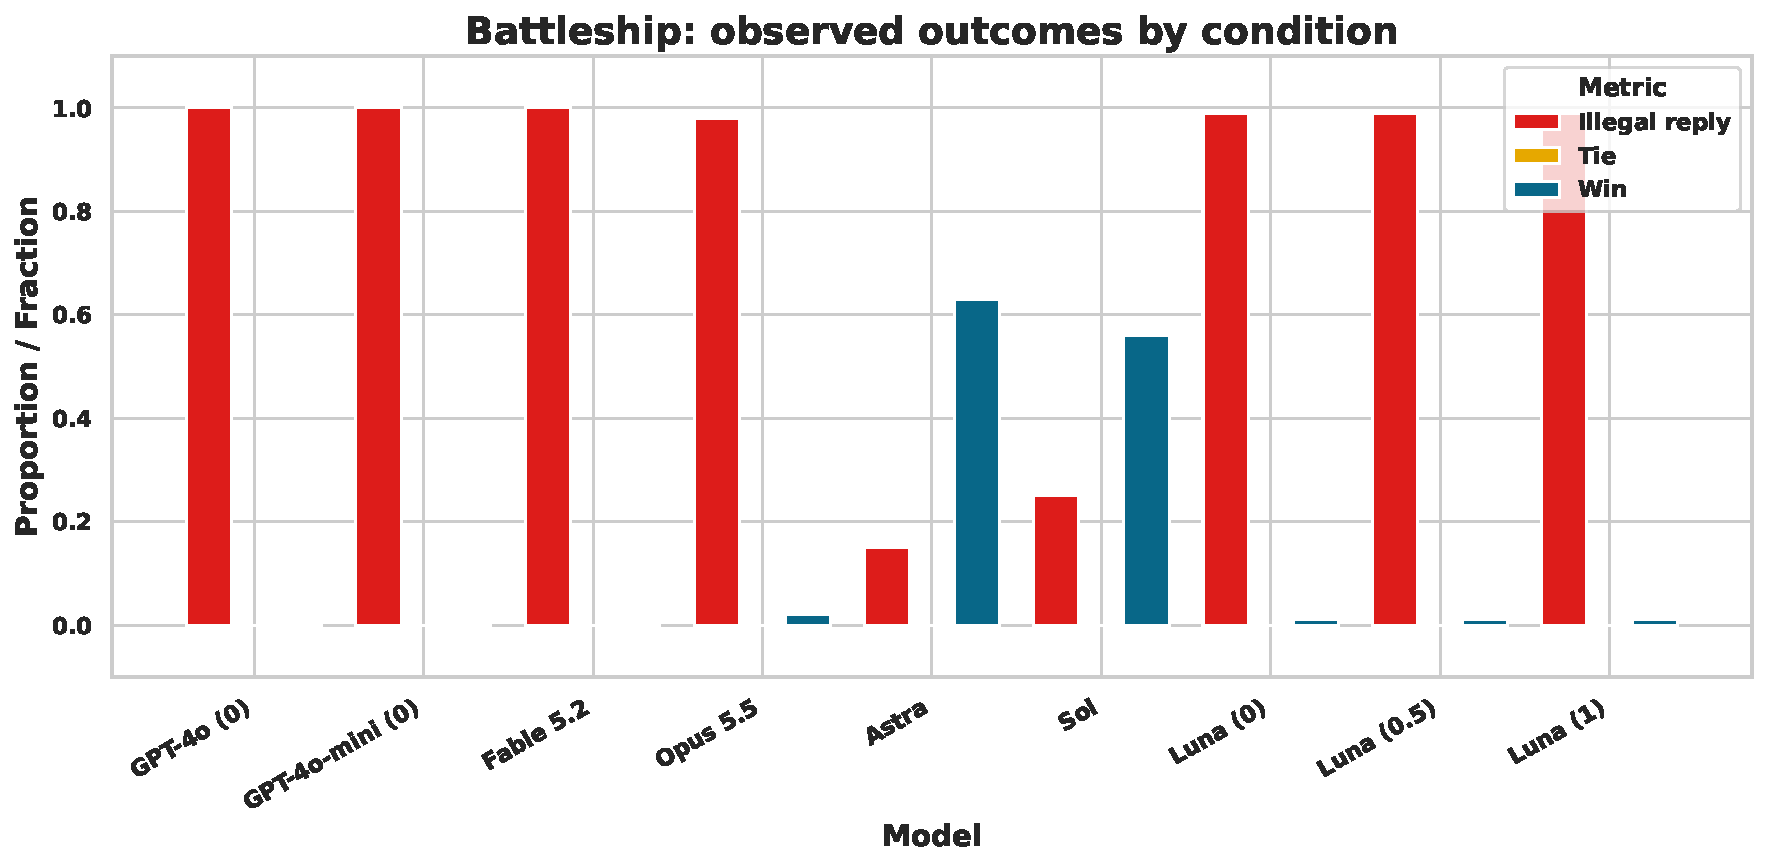
\includegraphics[width=.95\linewidth]{complete/model_comparison_battleship.pdf}
\caption{Battleship outcomes by condition. Win, tie, and illegal-reply fractions use all 100 games. Illegal replies are only one component of total losses. Categorical conditions are shown as bars, without implying a temporal trajectory.}\label{fig:battleship}
\end{figure}
\begin{figure}[tbp]\centering
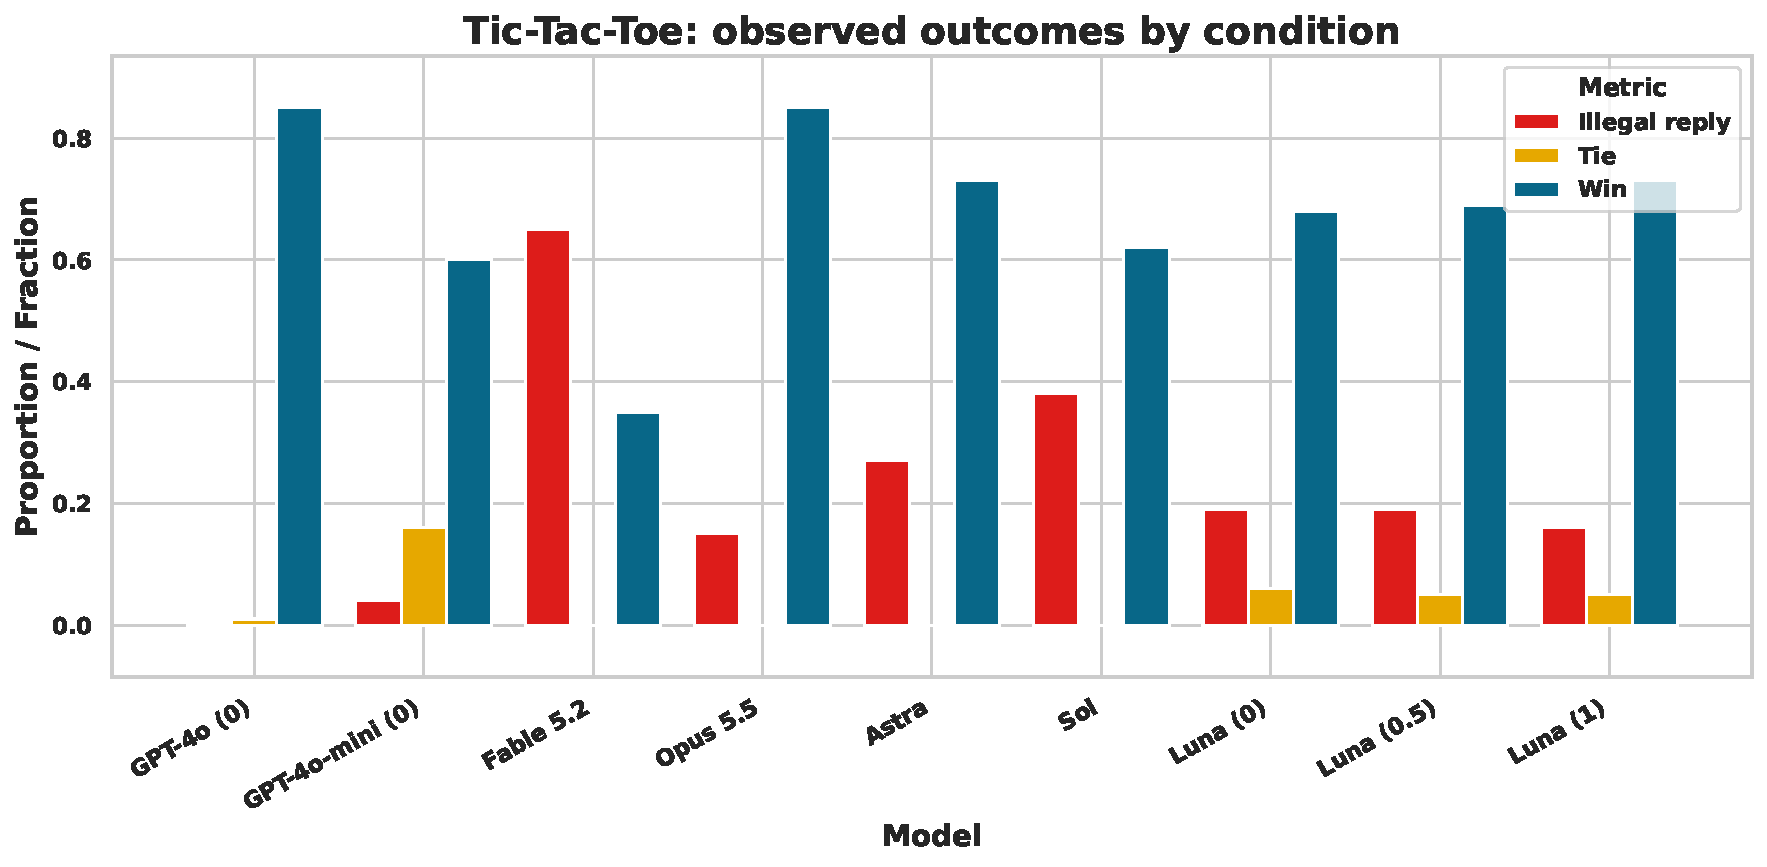
\includegraphics[width=.95\linewidth]{complete/model_comparison_tictactoe.pdf}
\caption{Tic-Tac-Toe outcomes in 100 games per condition.}\label{fig:ttt}
\end{figure}
\begin{figure}[tbp]\centering
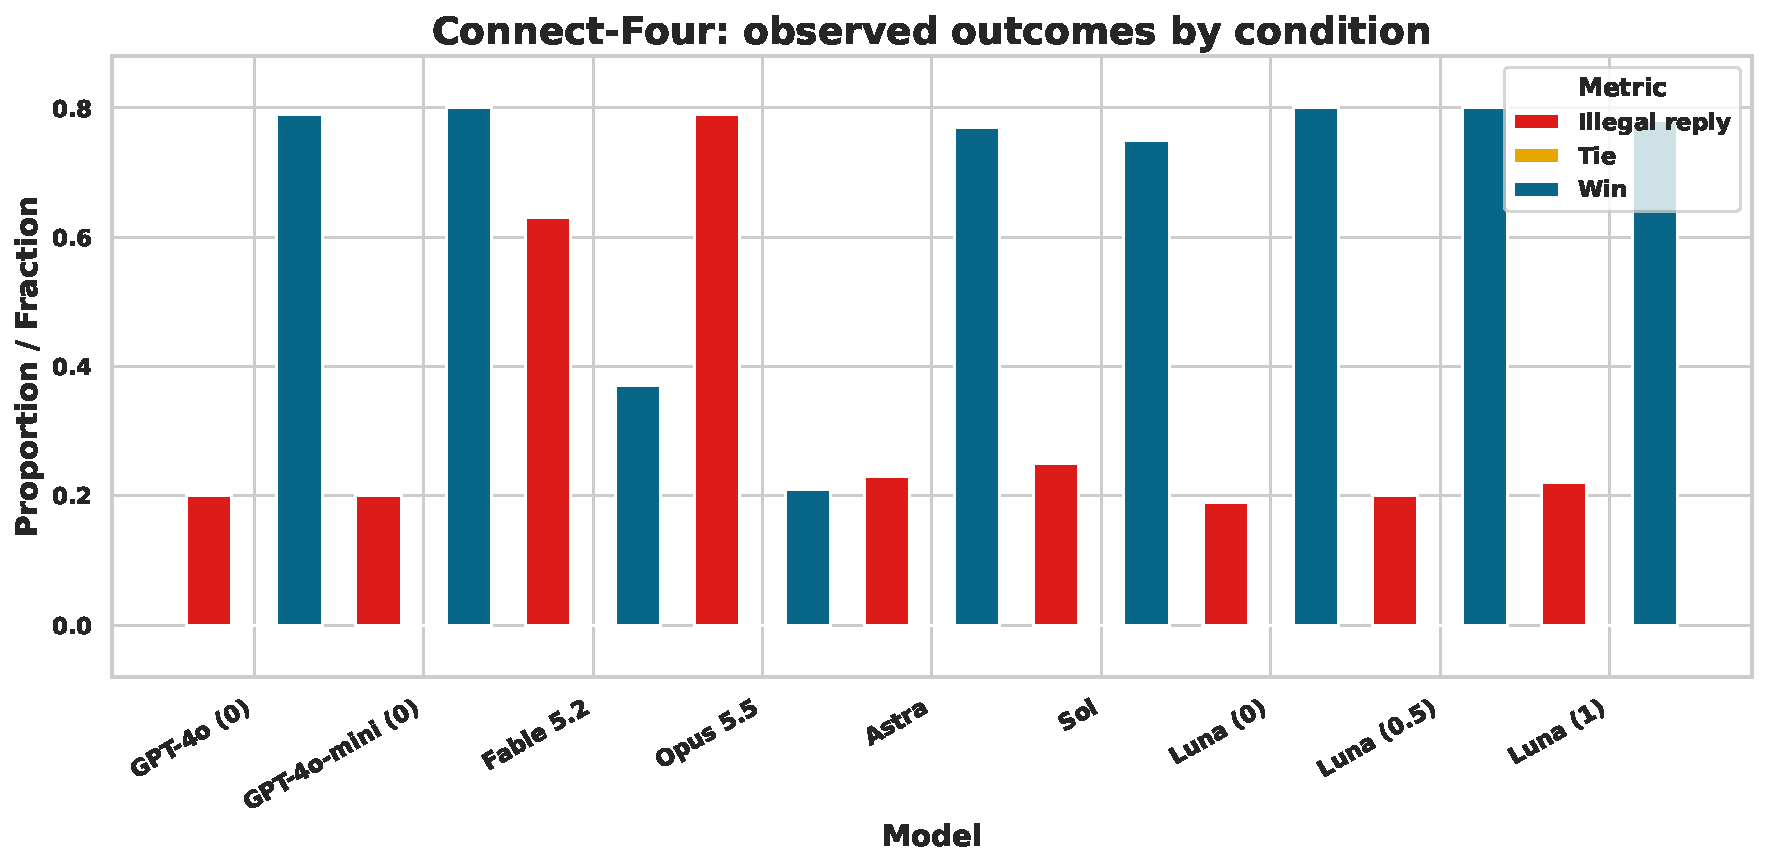
\includegraphics[width=.95\linewidth]{complete/model_comparison_connectfour.pdf}
\caption{Connect-Four outcomes in 100 games per condition. The opponent samples legal columns uniformly.}\label{fig:c4}
\end{figure}

\subsection*{Shape recognition and spatial construction}
Shape recognition is near ceiling for several later conditions, while GPT-4o-mini at temperature 0 is substantially less accurate (Table~\ref{tab:scores}). The per-class breakdown identifies whether a score reflects failures on one shape rather than uniformly weak classification. LCL validity and generation assess different operations. Under the explicit rules, GPT-4o judges 98 of 100 constructs correctly and generates 100 valid three-piece lists. Astra and Sol reach 100 on both tasks. Fable and Opus each generate 100 valid lists while judging only 53 and 66 of the validity items correctly. GPT-4o-mini judges 50 correctly and generates no valid list. These differences show why the two operations should be reported separately. The reported LCL results all use the explicit geometry and strict three-piece generation parser; the earlier under-specified-prompt results are not used in this comparison.

\begin{figure}[tbp]\centering
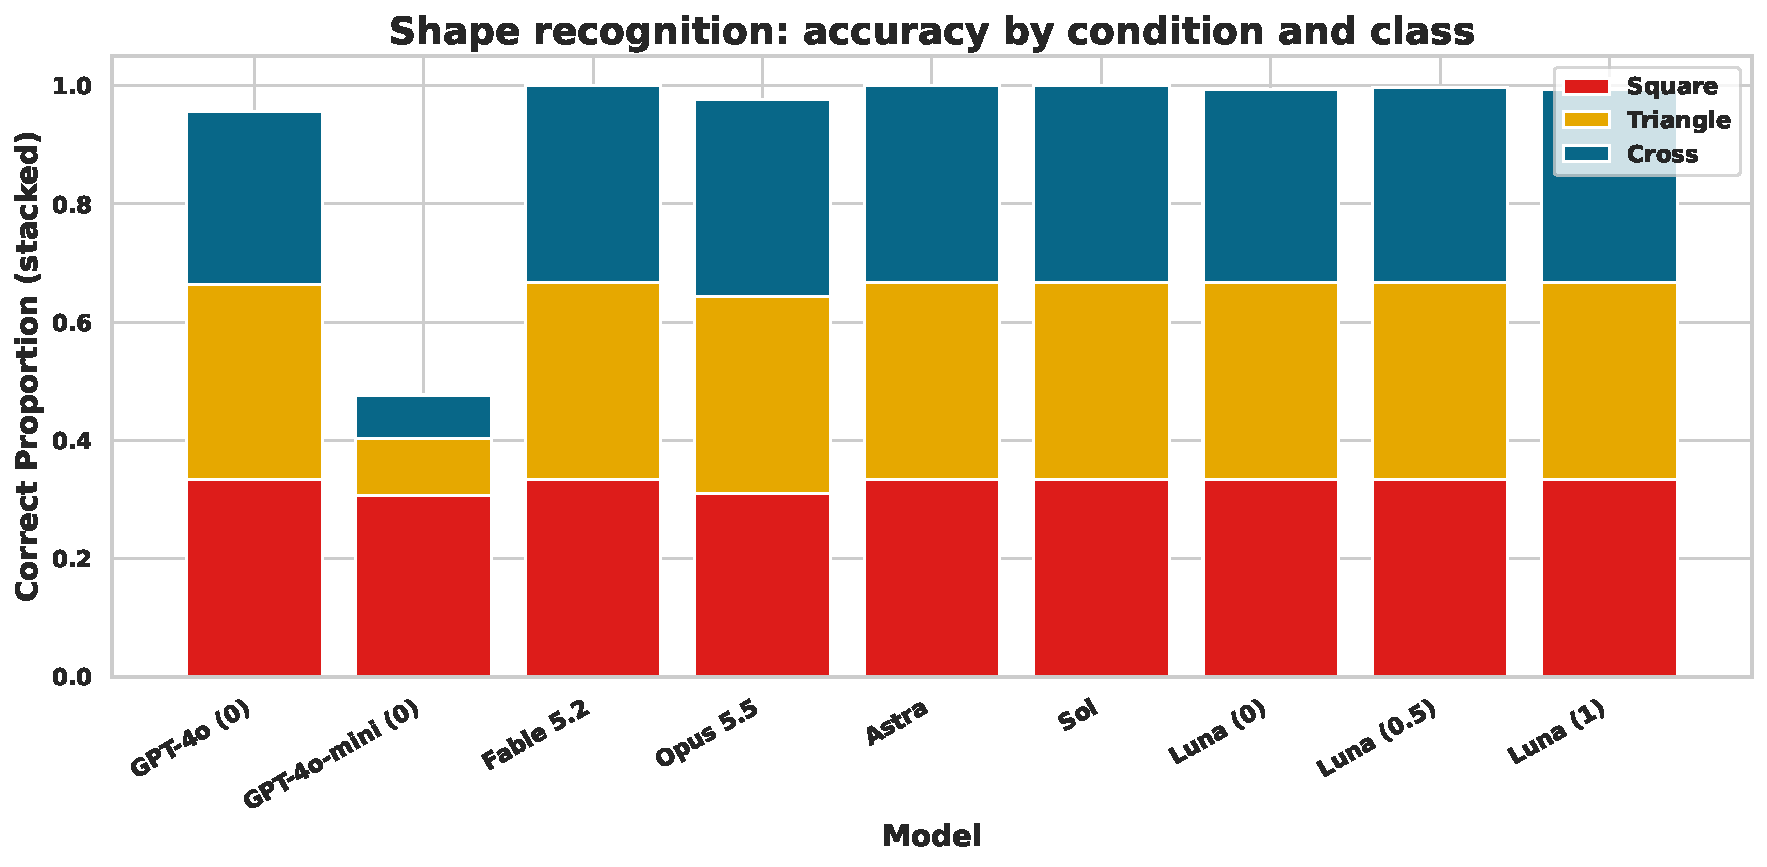
\includegraphics[width=.95\linewidth]{complete/model_comparison_shapes.pdf}
\caption{Shape recognition accuracy across 300 boards per condition. Each stacked component is that class's correct fraction divided by three, so the total is overall accuracy.}\label{fig:shapes}
\end{figure}
\begin{figure}[tbp]\centering
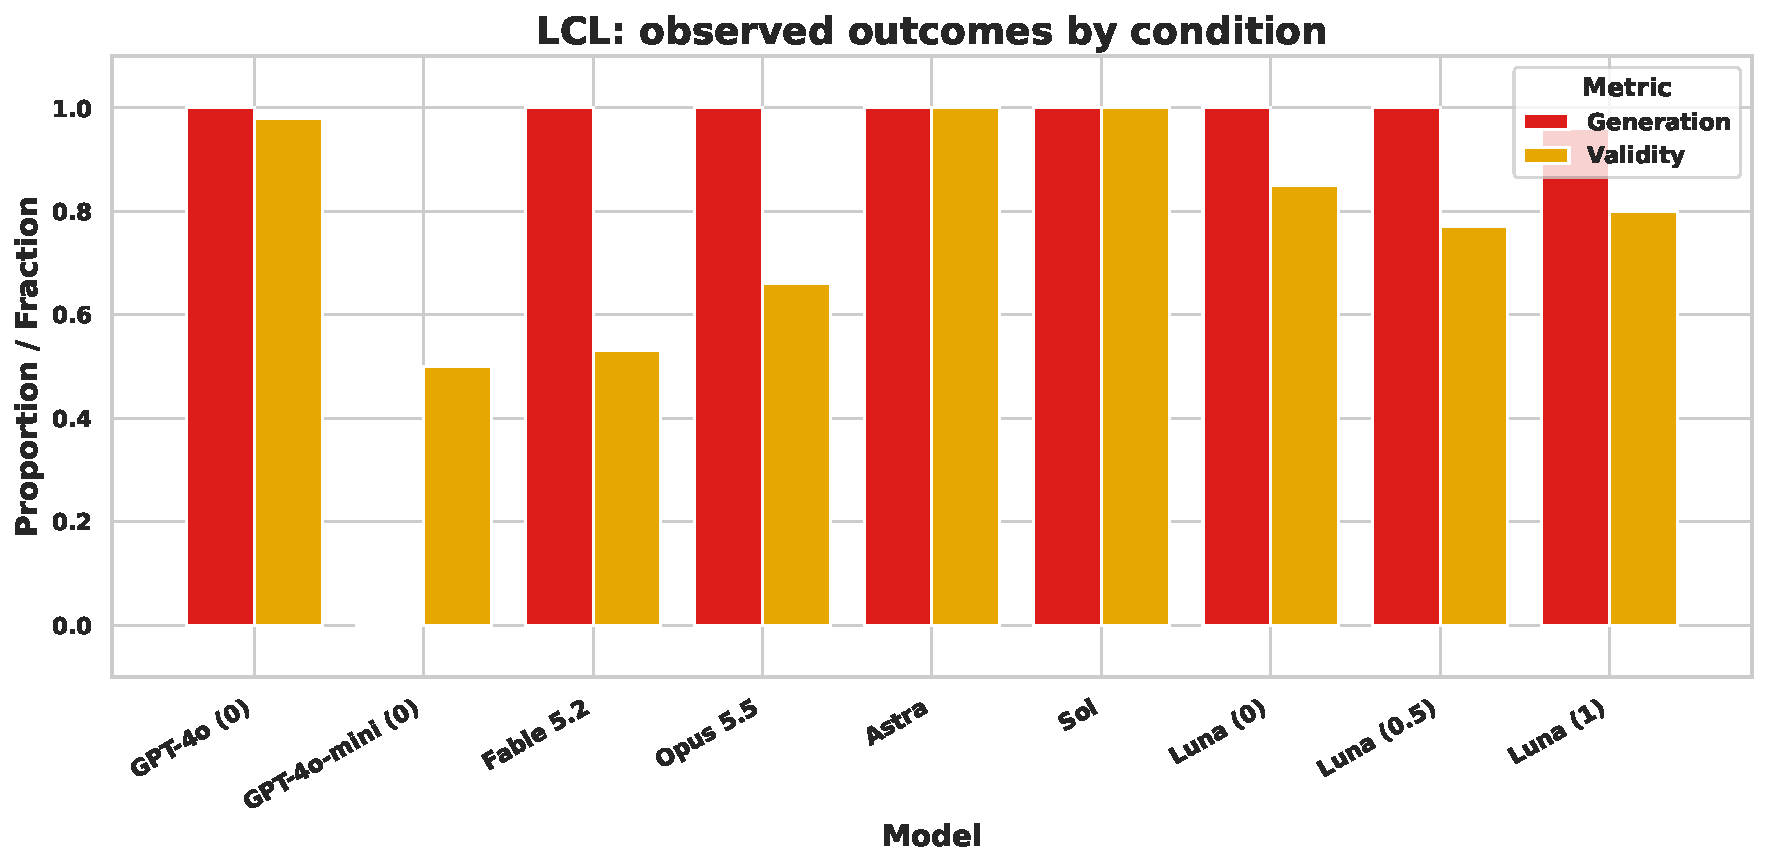
\includegraphics[width=.95\linewidth]{complete/model_comparison_lcl.pdf}
\caption{LCL validity and three-piece generation success under explicit geometry. Each task uses 100 trials per condition. All replies, including malformed lists, contribute to the denominator.}\label{fig:lcl}
\end{figure}

\subsection*{Molecular transcription and the overall summary}
\begin{table}[tbp]
\centering
\small
\resizebox{\textwidth}{!}{%
\begin{tabular}{lrrrrrr}
\toprule
Condition & Correct & Other incorrect & Invalid & All-reply accuracy & Conditional accuracy & Penalized similarity \\
\midrule
GPT-4o (0) & 5 & 92 & 3 & 5.00 & 5.15 & 0.220 \\
GPT-4o-mini (0) & 1 & 89 & 10 & 1.00 & 1.11 & 0.072 \\
Fable 5.2 & 45 & 30 & 25 & 45.00 & 60.00 & 0.207 \\
Opus 5.5 & 20 & 53 & 27 & 20.00 & 27.40 & -0.070 \\
Astra & 100 & 0 & 0 & 100.00 & 100.00 & 1.000 \\
Sol & 99 & 1 & 0 & 99.00 & 99.00 & 0.995 \\
Luna (0) & 4 & 77 & 19 & 4.00 & 4.94 & 0.007 \\
Luna (0.5) & 3 & 82 & 15 & 3.00 & 3.53 & 0.030 \\
Luna (1) & 2 & 70 & 28 & 2.00 & 2.78 & -0.118 \\
\bottomrule
\end{tabular}}
\caption{GtS results from complete retained responses, with 100 drawings per condition. All-reply accuracy is correct/100 and is the primary score. Conditional accuracy excludes the invalid-SMILES sentinel and is secondary. Similarity averages the Dice score with a value of $-1$ for that sentinel; empty or overlength replies instead receive 0. Both accuracy columns are percentages.}
\label{tab:gts}
\end{table}

Astra correctly transcribes \AstraGts{} of the 100 drawings and Sol \SolGts{}. Fable identifies \FableGts{}, Opus \OpusGts{}, GPT-4o \FourOGts{}, and GPT-4o-mini \FourMiniGts{}. Luna identifies four, three, and two drawings at temperatures 0, 0.5, and 1, respectively. These are unconditional success counts from complete newly retained replies. A correct graph can be returned through a non-identical string: canonicalization checks equivalence rather than literal target-string reproduction.

Astra and Sol have overall descriptive scores of \AstraOverall\% and \SolOverall\%. These averages summarize the stated task mixture and inference conditions. They do not establish a stable ranking across other task weights, prompts, representations, or sampling runs.

\begin{figure}[tbp]\centering
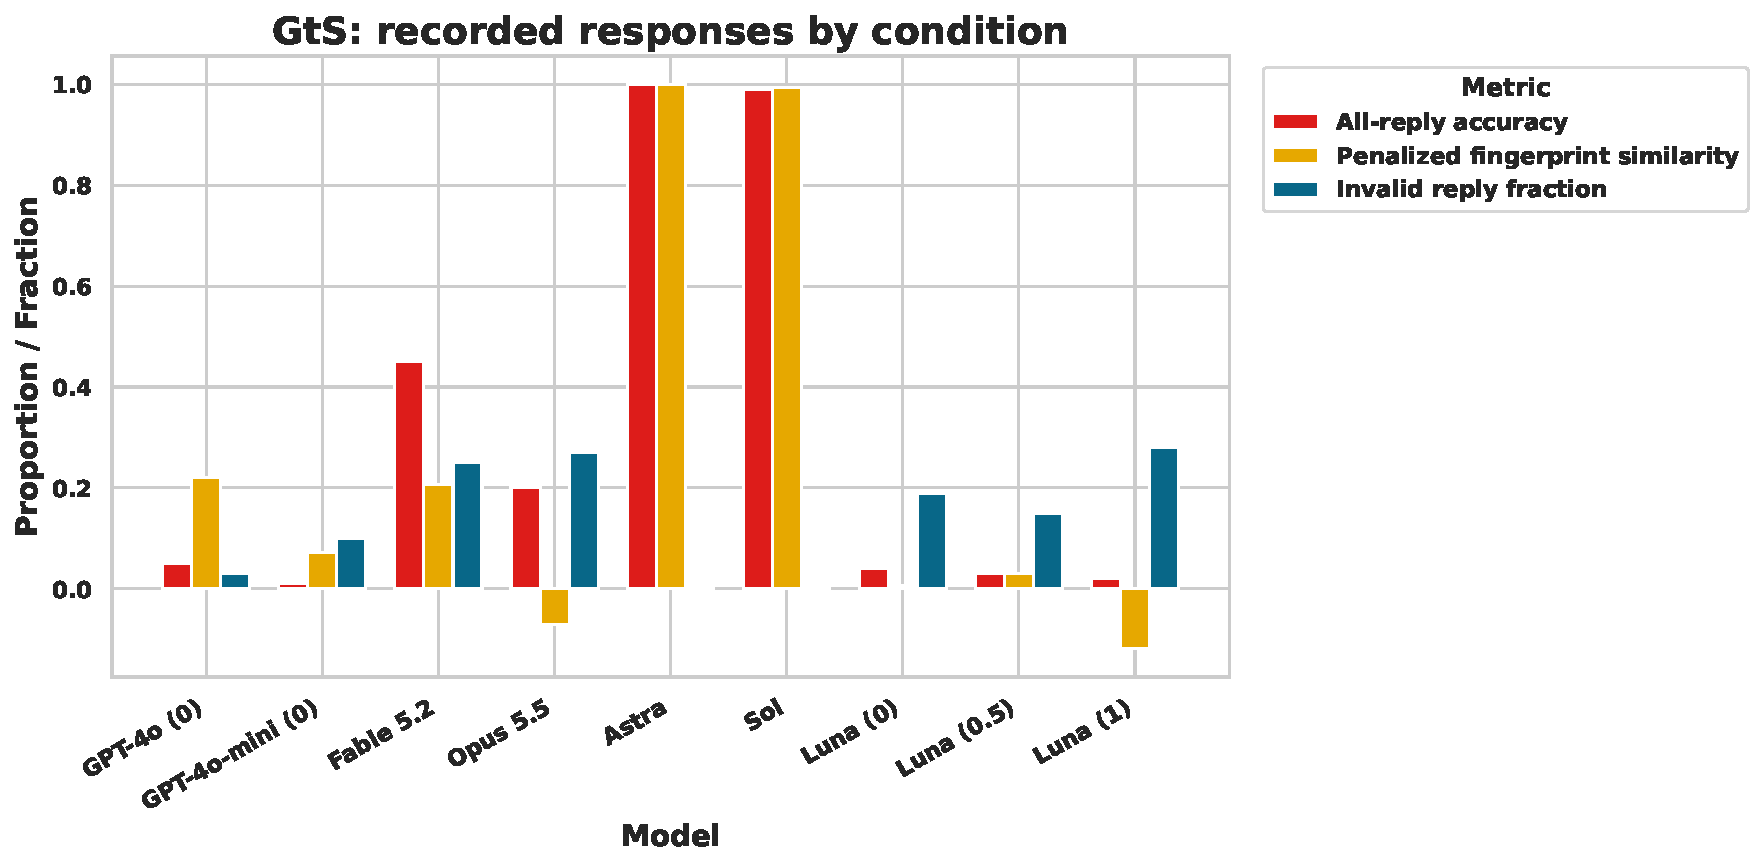
\includegraphics[width=.95\linewidth]{complete/model_comparison_molecules.pdf}
\caption{GtS all-reply accuracy, invalid-parser reply fraction, and penalized fingerprint similarity. The last quantity may be negative because invalid-parser replies receive $-1$.}\label{fig:gts}
\end{figure}
\begin{figure}[tbp]\centering
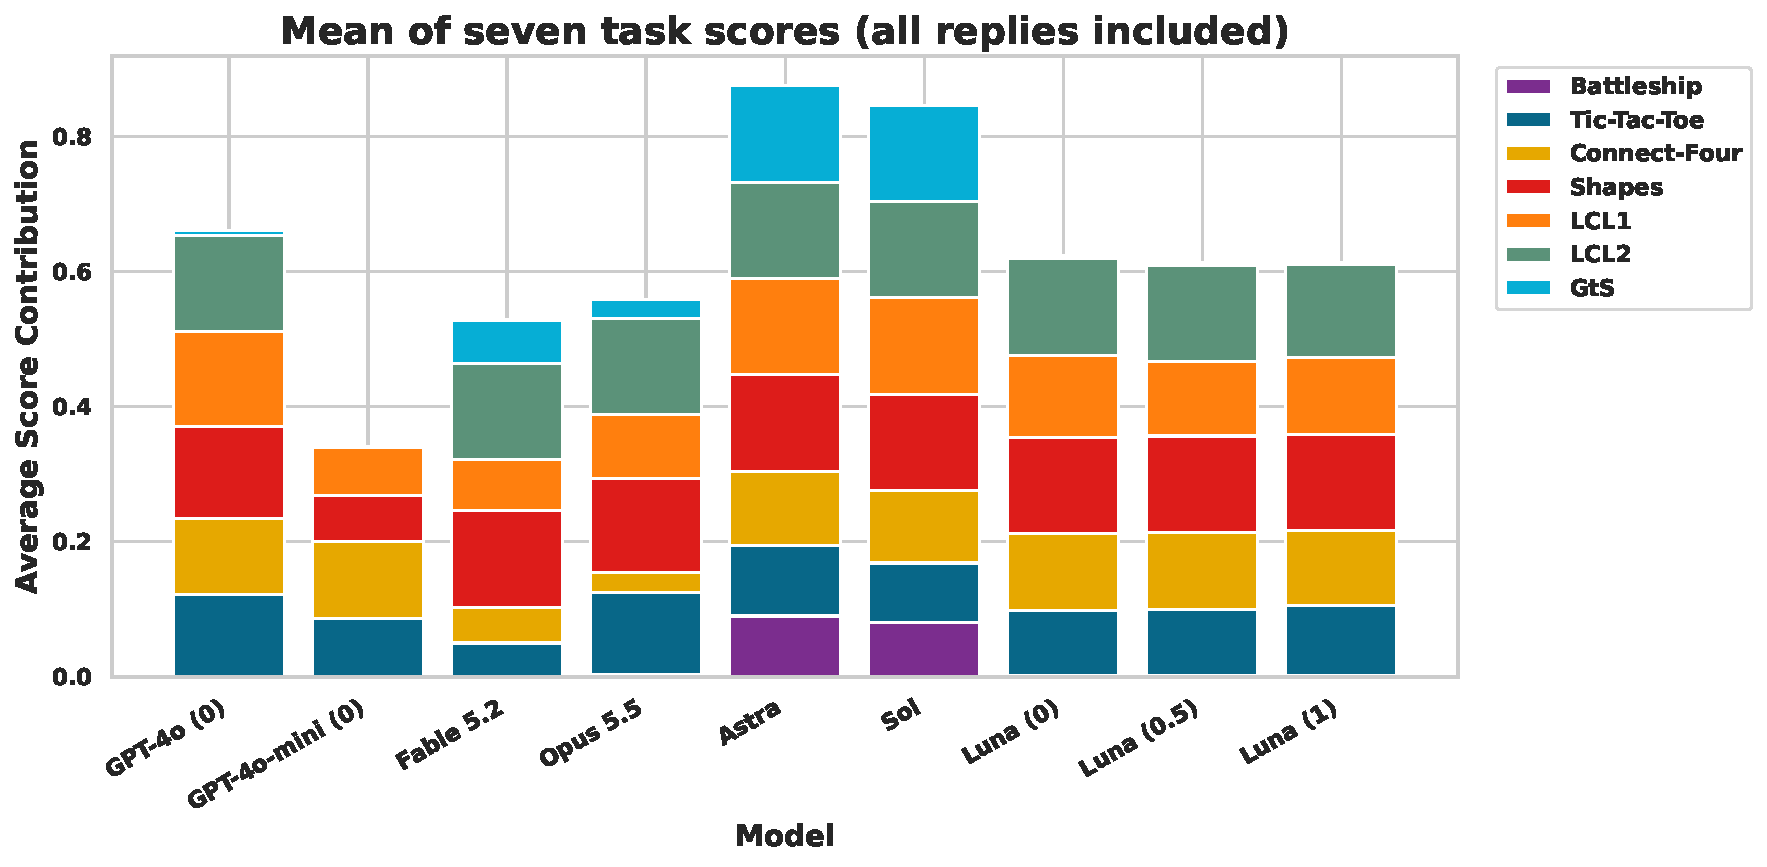
\includegraphics[width=.95\linewidth]{complete/merged_metrics_per_model.pdf}
\caption{Equal-weight mean of seven task scores for each actual condition. Every component includes invalid replies as failures. Luna's temperatures remain separate conditions.}\label{fig:overall}
\end{figure}

\section*{Discussion}
The main empirical finding is uneven reliability across tasks under a specified interface. High molecular-transcription or shape-classification performance coexists with imperfect gameplay, and some low board-game scores largely reflect failure to produce an accepted move. This supports task-specific validation rather than extrapolating from a fluent explanation or a strong score elsewhere.

The later transcription results also qualify a broad claim of persistent failure on spatial or chemical tasks. Astra and Sol perform strongly on these small molecular graphs. That success deserves to be reported without being extended to untested chemical applications. Conversely, failure on GtS does not invalidate results from molecular property prediction or laboratory automation, which assess different workflows \cite{jablonka2024leveraging,boiko2023autonomous}.

The results do not distinguish memorization, learned procedures, state representations, or other internal explanations. Generated inputs do not eliminate related training exposure, and fixed model parameters do not rule out input-dependent computation. Prior probing and intervention studies provide evidence about particular sequence models \cite{li2023emergent,nanda2023linear}; the behavioral records here neither establish nor refute analogous mechanisms in these proprietary models. Explanations should be evaluated alongside execution without treating either success or failure as a complete mechanistic account.

\subsection*{Limitations}
The evaluation covers a narrow set of textual representations, small graphs, and one family of random opponents. First-player advantage and simple move biases can yield wins against that opponent. No matched strategic-strength ordering or optimal Battleship baseline is established. The board-game prompts score the whole reply, whereas GtS permits the specified prefix removal and canonicalizes molecular strings. These parser choices are part of the task definitions and can affect performance.

The reported scores do not establish robustness to alternative prompts, demonstrations, external tools, search, or feedback. Such methods can change computation and information during inference and require direct evaluation \cite{DBLP:journals/corr/abs-2201-11903,yao2023treethoughtsdeliberateproblem}. The present zero-shot conditions are not a general test of those approaches.

Repeated openings and construction instructions limit the independence and diversity of the trials. Tactical-error rates are conditional on reaching a position and making an accepted move: an early illegal reply can produce a low tactical count without competent play. We therefore interpret those rates together with outcomes and accepted-move counts. Best observed settings and descriptive aggregate differences should not be treated as statistically established model rankings.

Training corpora are unavailable, and some problem families are well known. Newly generated items therefore cannot certify out-of-training-distribution generalization. Model aliases, provider implementations, and sampling can change future live outputs. Retaining the actual inputs and replies makes the reported scoring reproducible without claiming that a future model call will produce the same answer.

\subsection*{Conclusions}
\texttt{ChildPlay} provides explicit, reproducible behavioral scoring for seven tasks. The complete selected records show both substantial successes and persistent task-specific failures. The practical implication is to validate the action or structural answer required by an application, while keeping claims about internal mechanisms and broad competence proportional to the evidence.

\section*{Data and Code Availability}
Source code, frozen inputs, complete selected response ledgers, and reproduction commands are available in the \href{https://github.com/BlueVelvetSackOfGoldPotatoes/child-play}{ChildPlay repository}. The first-paper entry point is \path{utils/render_paper.py}; machine-readable metrics and source hashes are in \path{paper/complete/metrics.json} and \path{paper/complete/provenance.json}. The original historical records and superseded draft are retained separately and are not used to fill the current comparison. GtS generation and scoring code are included in the source release.

\section*{Author Contributions}
All authors contributed equally.

\section*{Acknowledgments}
The evaluation of Fable 5.2, Opus 5.5, Astra, Sol, and Luna was carried out at and supported by \href{https://hellolupa.com}{Lupa Labs}. MarvinSketch version 24.4.2 was used to prepare chemical structure schemes.

\bibliography{main,childplay_review_references}
\clearpage
\appendix
\section{Detailed results and instructions}
\begin{table}[tbp]
\centering
\small
\resizebox{\textwidth}{!}{%
\begin{tabular}{lrrrr}
\toprule
Condition & Wins & Losses & Ties & Illegal-reply losses \\
\midrule
GPT-4o (0) & 0 & 100 & 0 & 100 \\
GPT-4o-mini (0) & 0 & 100 & 0 & 100 \\
Fable 5.2 & 0 & 100 & 0 & 100 \\
Opus 5.5 & 2 & 98 & 0 & 98 \\
Astra & 63 & 37 & 0 & 15 \\
Sol & 56 & 44 & 0 & 25 \\
Luna (0) & 1 & 99 & 0 & 99 \\
Luna (0.5) & 1 & 99 & 0 & 99 \\
Luna (1) & 1 & 99 & 0 & 99 \\
\bottomrule
\end{tabular}}
\caption{Battleship outcomes in 100 games against a random legal opponent. Illegal-reply losses are included in losses, not added to them.}
\label{tab:battleship}
\end{table}

\begin{table}[tbp]
\centering
\small
\resizebox{\textwidth}{!}{%
\begin{tabular}{lrrrr}
\toprule
Condition & Wins & Losses & Ties & Illegal-reply losses \\
\midrule
GPT-4o (0) & 85 & 14 & 1 & 0 \\
GPT-4o-mini (0) & 60 & 24 & 16 & 4 \\
Fable 5.2 & 35 & 65 & 0 & 65 \\
Opus 5.5 & 85 & 15 & 0 & 15 \\
Astra & 73 & 27 & 0 & 27 \\
Sol & 62 & 38 & 0 & 38 \\
Luna (0) & 68 & 26 & 6 & 19 \\
Luna (0.5) & 69 & 26 & 5 & 19 \\
Luna (1) & 73 & 22 & 5 & 16 \\
\bottomrule
\end{tabular}}
\caption{Tic-Tac-Toe outcomes in 100 games against a random legal opponent. Illegal-reply losses are included in losses, not added to them.}
\label{tab:tictactoe}
\end{table}

\begin{table}[tbp]
\centering
\small
\resizebox{\textwidth}{!}{%
\begin{tabular}{lrrrr}
\toprule
Condition & Wins & Losses & Ties & Illegal-reply losses \\
\midrule
GPT-4o (0) & 79 & 21 & 0 & 20 \\
GPT-4o-mini (0) & 80 & 20 & 0 & 20 \\
Fable 5.2 & 37 & 63 & 0 & 63 \\
Opus 5.5 & 21 & 79 & 0 & 79 \\
Astra & 77 & 23 & 0 & 23 \\
Sol & 75 & 25 & 0 & 25 \\
Luna (0) & 80 & 20 & 0 & 19 \\
Luna (0.5) & 80 & 20 & 0 & 20 \\
Luna (1) & 78 & 22 & 0 & 22 \\
\bottomrule
\end{tabular}}
\caption{Connect-Four outcomes in 100 games against a random legal opponent. Illegal-reply losses are included in losses, not added to them.}
\label{tab:connectfour}
\end{table}

\begin{table}[tbp]
\centering
\small
\resizebox{\textwidth}{!}{%
\begin{tabular}{lrrrr}
\toprule
Condition & Square & Triangle & Cross & Overall \\
\midrule
GPT-4o (0) & 100.00 & 99.00 & 88.00 & 95.67 \\
GPT-4o-mini (0) & 92.00 & 29.00 & 22.00 & 47.67 \\
Fable 5.2 & 100.00 & 100.00 & 100.00 & 100.00 \\
Opus 5.5 & 93.00 & 100.00 & 100.00 & 97.67 \\
Astra & 100.00 & 100.00 & 100.00 & 100.00 \\
Sol & 100.00 & 100.00 & 100.00 & 100.00 \\
Luna (0) & 100.00 & 100.00 & 98.00 & 99.33 \\
Luna (0.5) & 100.00 & 100.00 & 99.00 & 99.67 \\
Luna (1) & 100.00 & 100.00 & 98.00 & 99.33 \\
\bottomrule
\end{tabular}}
\caption{Shape recognition percentages: 100 boards per class and condition. Overall uses all 300 boards.}
\label{tab:shapes}
\end{table}

\clearpage
\section{Accepted-move and tactical analyses}
The same corrected counters are used for every condition. Bar heights are rates per retained game, with 100 games in every selected condition. A successful block is excluded from the missed-block count, and a newly created threat is excluded from the missed-win count. Complete per-condition move heatmaps and their counts accompany the electronic artifacts.
\begin{figure}[tbp]\centering
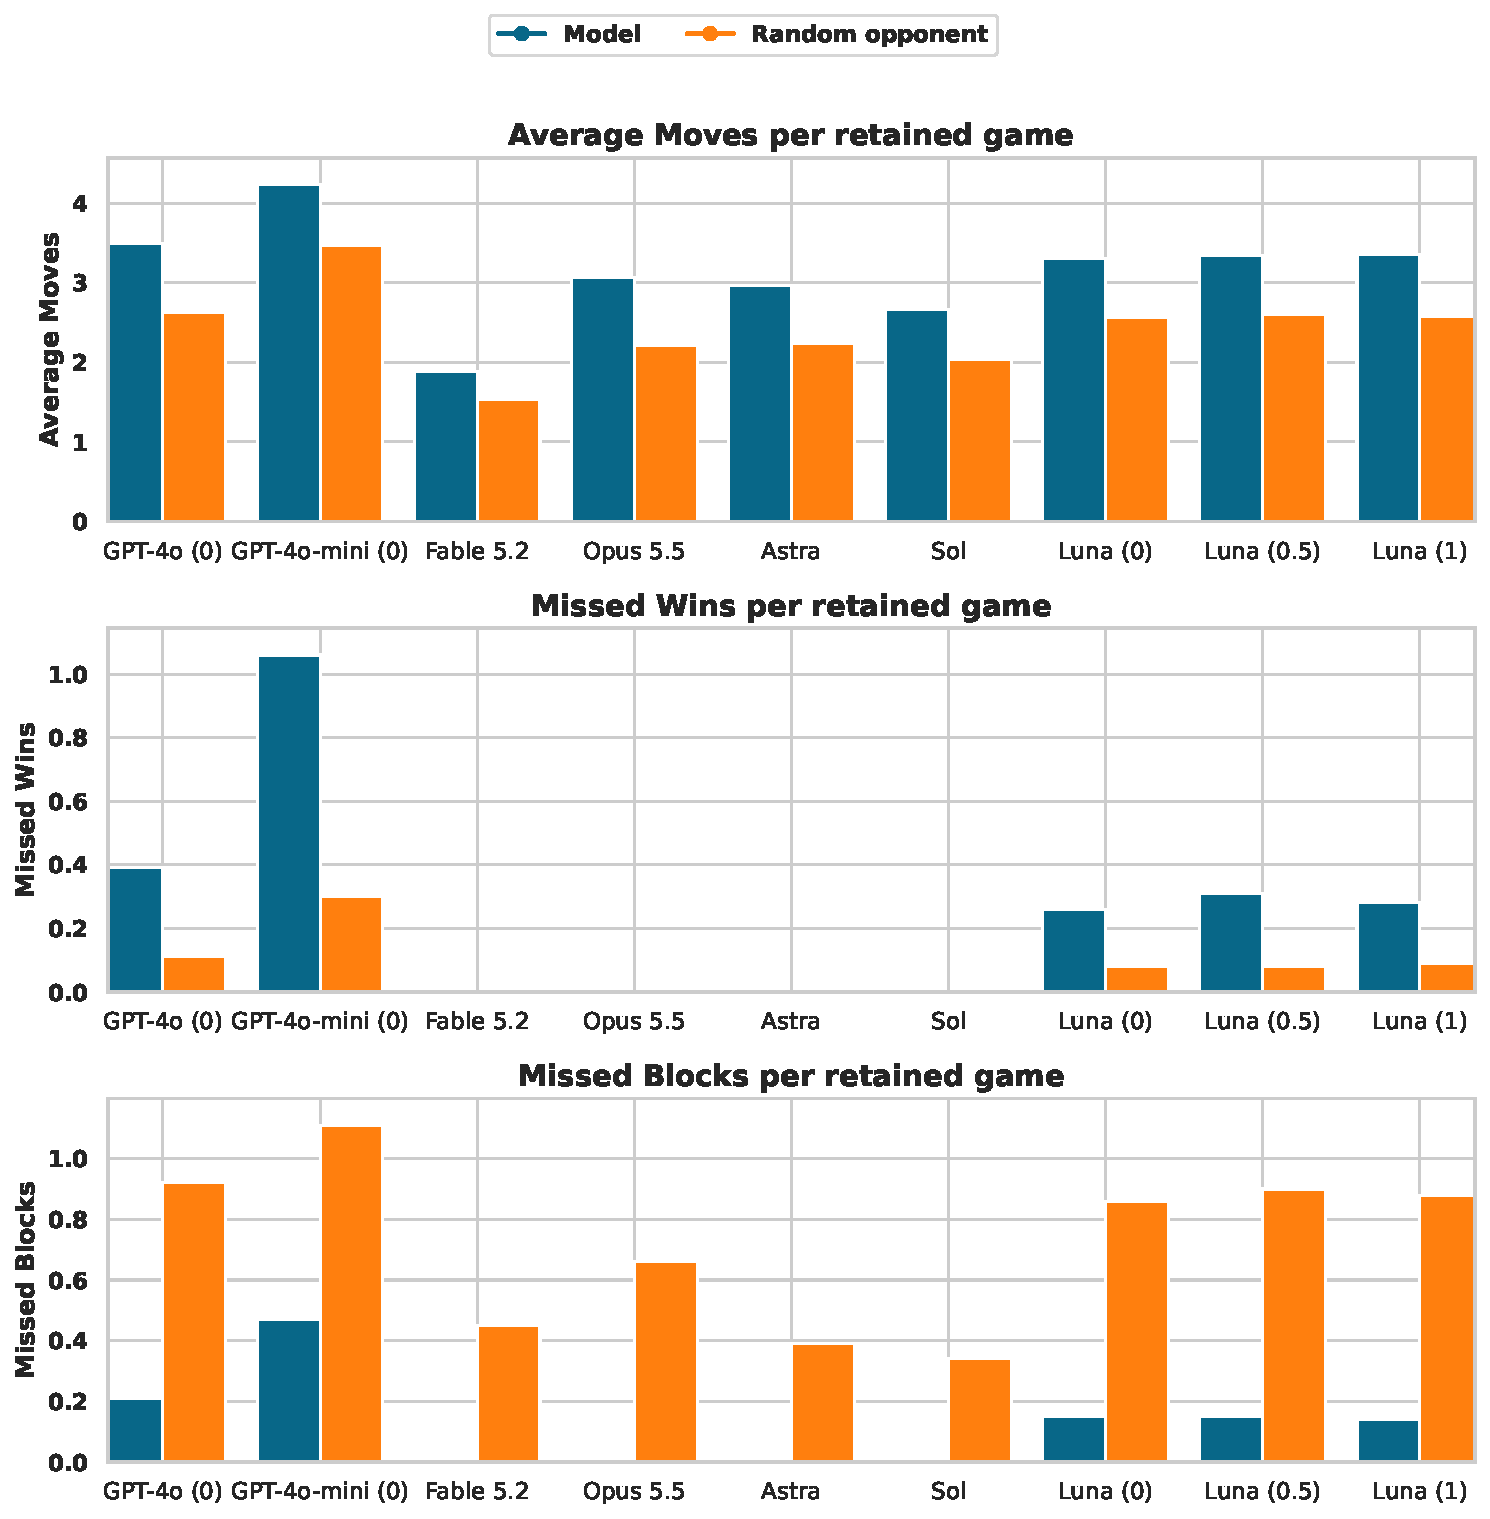
\includegraphics[width=.98\linewidth,height=.8\textheight,keepaspectratio]{complete/tictactoe_tactics.pdf}
\caption{Tic-Tac-Toe accepted moves, missed immediate wins, and missed blocks per retained game, for the model and its random opponent.}\label{fig:ttt-tactics}
\end{figure}
\begin{figure}[tbp]\centering
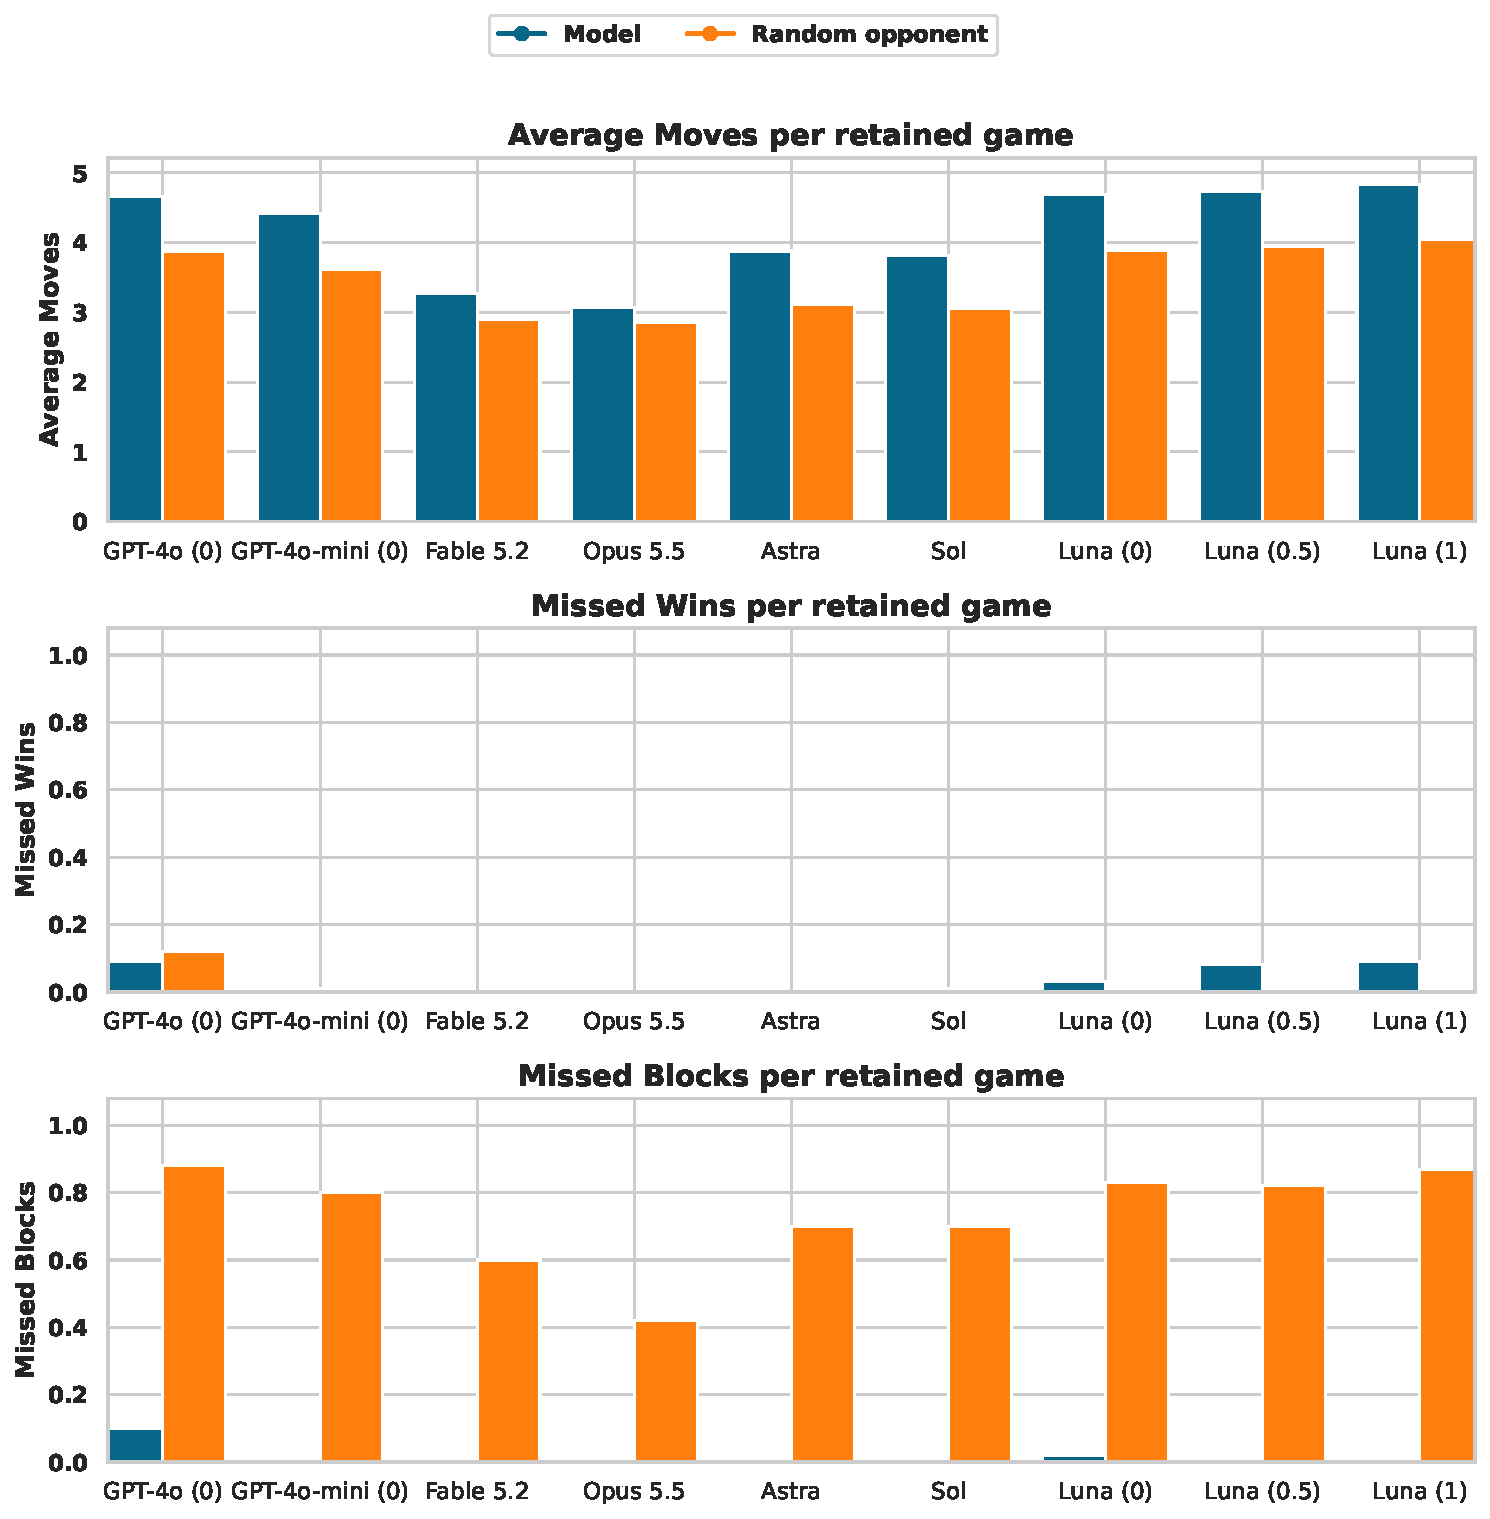
\includegraphics[width=.98\linewidth,height=.8\textheight,keepaspectratio]{complete/connectfour_tactics.pdf}
\caption{Connect-Four accepted moves, missed immediate wins, and missed blocks per retained game.}\label{fig:c4-tactics}
\end{figure}
\clearpage
\section{Prompt and input provenance}
Each board-game system message is the game instruction prefixed with ``You are a player in a game of [name].'' The user turn names Player 1, supplies its current observation, and ends with ``My move is:''. The exact shared instructions and task inputs are retained in the frozen stimulus files identified by their hashes. LCL uses the instruction revision that explicitly specifies four occupied x positions, one-level adjacency, global connectivity, and the exact requested reply. GtS uses the molecular instruction and fixed extraction prefix in the published runner. The reproduction script reads these inputs and the selected original replies; it does not call a model, generate substitute replies, or infer missing records.
\end{document}
